\chapter{Problematika vývoje rozšíření pro VS Code}

\section{Visual Studio Code}
Visual Studio Code \cite{VSCODE_2020} je editor zdrojového kódu vytvořený společností Microsoft pro operační Windows, Linux a MacOS. Nabízí spoustu užitečných funkcí, mezi které patří podpora ladění kodu, zvýrazňování syntaxe, automatické doplňování a našeptávání kódu, atd… Naším cílem je integrovat většinu těchto funkcí a možností do finálního rozšíření.

\section{Typescript}
TypeScript \cite{TypeScript_wikipedia_2020} je open-source programovací jazyk vyvinutý společností Microsoft. Jedná se o nádstavbu nad jazykem JavaScript,
která jej rozšiřuje o statické typování a další atributy, které známe z objektově orientovaného programování jako jsou třídy, moduly a další. Samotný kód psaný v jazyce TypeScript se kompiluje
do jazyka JavaScript. Jelikož je tento jazyk nádstavbou nad JavaScriptem, je každý JavaScript kód automaticky validním TypeScript kódem.

\section{Komponenty potřebné pro vytvoření rozšíření}
Předtím, než začneme pracovat na samotném rozšíření, je potřeba obstarat několik důležitých nastrojů a komponent, jenž jsou klíčové při vývoji.
\subsection{Gramatika}
Jako první je potřeba definovat popis jazyka MonkeyC. V našem případě je jazyk popsán prostřednictvím bezkontextové gramatiky, která formálně definuje syntax (pravidla) jazyka.

\begin{figure}
	\centering
	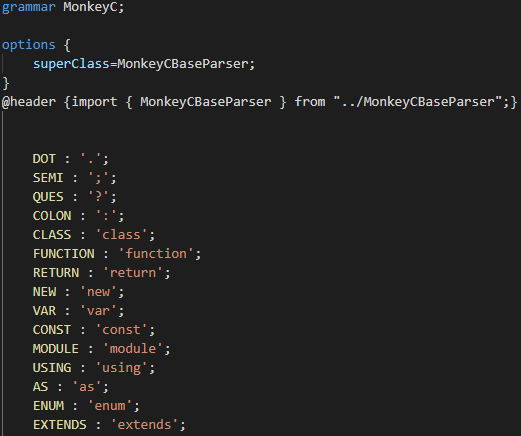
\includegraphics[scale=0.8]{images/grammar}
	\caption{ukázka hlavičky gramatiky MonkeyC.g4 pro popis jazyka}
	\label{img:grammar}
\end{figure}

Na obrázku mužeme vidět prvních pár řádků gramatiky pro MonkeyC. Gramatika obsahuje spoustu známých klíčových slov, nebo-li tokenů, např. "CLASS", "FUNCTION", "USING", atd...

\subsection{Java}
Jelikož je ANTLR psán v Javě, je potřeba ji nainstalovat na naše zařízení, přičemž se požaduje verze 1.6 nebo vyšší. Poté již stačí stáhnout akualní ANTLR jar, což je momentálně "antlr-4.8-complete.jar".

\subsection{Parser a Lexer}
\textbf{lexer} - lexer (nebo také tokinizér) "rozdělí" text na vstupu (v našem případě MonkeyC kód) na tokeny. \cite{ANTLR_PG_20} \\
\textbf{parser} - shora dolů prochází text na vstupu a porovnává jednotlivé řádky s pravidly obsažené v gramatice.\\
K vytvoření parseru a lexeru je potřeba spustit ANLTR nástroj, který s pomocí gramatiky tyto souboru vygeneruje. \cite{ANTLR_PG_20} \\

\begin{figure}
	\centering
	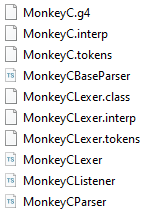
\includegraphics{images/generated_files}
	\\
	\caption{potřebné soubory vygenerované nástrojem ANTLR}
	\label{img:generated_files}
\end{figure}

\subsection{TestRig}
ANTLR poskytuje flexibilní testovací nástroj umístněný v runtime knihovně s názvem TestRig. TestRig dokáže poskytnout spoustu informací o tom, jak "recognizéry" (parser a lexer) zpracovávají InputStream ze vstupního souboru.\\
Nejjednodušší způsob ověření, zda gramatika rozpoznává vstup správně, je zobrazit si vygenerovaný syntaktický strom vizuálně.

\begin{figure}
	\centering
	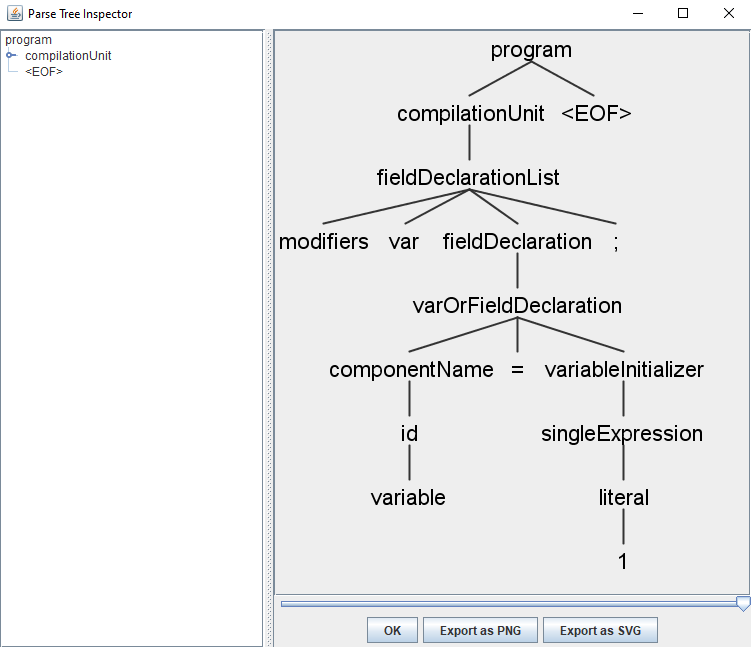
\includegraphics[scale=0.8]{images/ParseTreeInspector}
	\caption{"ParseTreeInspector" - vizuální podoba syntaktického stromu} 
	\label{img:ParseTreeInspector}
\end{figure}
Na obrázku můžeme detailně vidět jak parser vytvořil syntaktický strom a jak jsou jednotlivé části propojené. Strom začíná kořenem, jenž je v naší gramatice pojmenová, jako "program". Takto je kořen pojmenován při každém parsování. 

\endinput